\documentclass{book}

\usepackage[letterpaper]{geometry}
\usepackage{tgpagella}
\usepackage{amsmath}
\usepackage{amssymb}
\usepackage{amsthm}
\usepackage{tikz}
\usepackage{minted}
\usepackage{physics}
\usepackage{siunitx}
\usepackage{cite}
\usepackage{appendix}

\sisetup{detect-all}
\newtheorem{definition}{Definition}
\newtheorem{thm}{Theorem}
\newtheorem{lem}{Lemma}
\newtheorem{cor}{Corollary}
\newtheorem{prob}{Problem}
\newtheorem{exam}{Example}

\DeclareMathOperator{\Succ}{succ}
\DeclareMathOperator{\ar}{ar}
\newcommand{\hooktwoheadrightarrow}{\hookrightarrow\mathrel{\mspace{-15mu}}\rightarrow}

\AddToHook{cmd/section/before}{\clearpage}
\newcounter{philosophy}
\newenvironment{philosophy}{\refstepcounter{philosophy}\equation}{\tag{P\thephilosophy}\endequation}


\title{Algebra in Action}
\author{Duncan Wilkie}
\date{21 November 2023}

\begin{document}

\maketitle

\chapter*{Preface}

\textit{If you don't know algebra yet, skip to the roadmap; prefaces are directed at people assigning books.}
\vspace{20pt}

This book stems from a divine revelation I had while studying the frightening connections
between modules over field-valued polynomial rings and linear algebra in the wee hours of a morning my senior year of undergrad.
A Discord math friend had demonstrated the clear inadequacy of the geometric intuition for the determinant of a linear transformation,
and posed the question of an algebraic motivation for it.
Toiling over Dummit and Foote's approach to the structure theory of modules at the time, I quickly found the answer:
the product of the roots of the largest invariant factor of the underlying vector space, represented as a module over the polynomial ring
with coefficients in the underlying field where the transformation is replaced by an indeterminate.

This, alongside the spookily elementary proofs of the Jordan and rational canonical form theorems,
threatened my foundational understanding of operator theory, begotten of Axler's text \textit{par excellence}.
Surely, despite immediate motivation for the most fundamental concepts emerging from deepest depths, there's something more to the subject?
Could it really be, fundamentally, about polynomial rings?

Thinking over how one might deface Axler in this light brought a new perspective on the whole of algebra.
You're given a vector space $V$ over a field $F$, and a linear operator on it, $T$.
What can you do, without giving $V$ the standard agonizing vivisection?
Well, you can add any operator expression to any other, via pointwise addition in the vector space,
and you can borrow $V$'s scalar multiplication similarly.
You can also compose $T$ with itself, forming ``powers'' of $T$; this yields polynomials of the form
\[
  f_{0} + f_{1}T + f_{2}T^{2} + \cdots + f_{n}T^{n}, \text{ where} f_{i} \in F
\]
You then investigate the module action of evaluating the polynomial operators in the vector space, to overwhelming effect as described above.
The not-so-obvious part of this, at least \textit{ab initio}, is why we should consider opererator composition to be a kind of multiplication.
Pondering how to justify considering composition of $T$ as ``multiplication,'' it dawned on me that
\textit{every other multiplication is actually composition of endomorphisms}.

The attendant emotional consequences are witnessed in the figure.

\begin{center}
  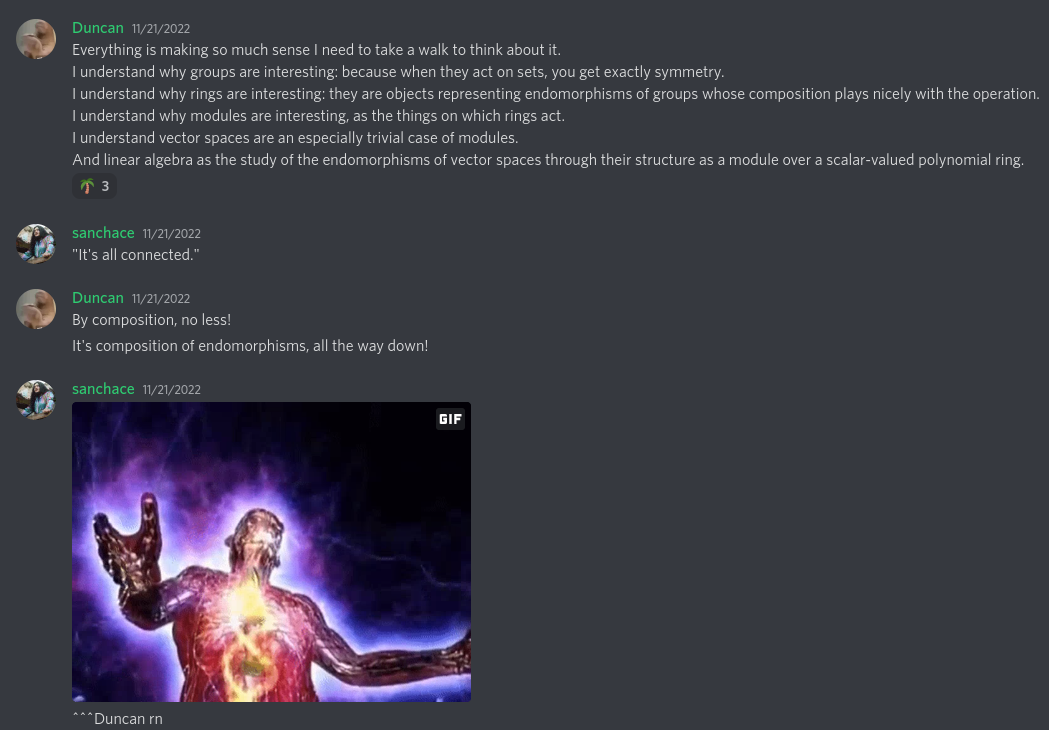
\includegraphics[scale=0.3]{fig/galaxy_brain.png}
\end{center}

This provided an intuitive justification for all my hard-won opinions on proper conventions (e.g. rings not rngs, 0 is a natural number),
explained definitions that seemed to fall from the sky (associativity, distributivity, rings are Abelian groups),
and provides a more palatable hint towards category theory than ``it's what we need to describe functors which are what we need to describe
natural transformations.''

Practically, this text seeks to be a first course in modern (abstract) algebra from a categorical perspective,
correcting the gaps in motivation left by the laudable recent treatments with the same goal. % TODO: Cite Aluffi and D\&F
The only prerequisite is an introduction to proofs class covering basic set theory, such as \textit{Book of Proof} or the first chapter of Munkres,
save the occasional footnote referencing some other area of mathematics that may be omitted with absolutely no impact on continuity.
The background formalism is sumarized in an appendix.

I produce also machine-verified proofs of each result, as an aid in my writing clear and concise arguments
and a recourse for the logically-minded reader peeved by my omission of trivial results, or suspicious of my wording.
They are in Lean 4, and are in print separately, in addition to freely distributed online.
I have made painstaking attempts to establish everything constructively, and any thus-intractable proof is distinguished by <a symbol> % TODO
and the nonconstructive step is identified in the text.

%%% Local Variables:
%%% mode: latex
%%% TeX-master: "../aia"
%%% End:


\chapter*{How to Read This Book}
I write this book to motivate.
As such, there's plenty of material in each chapter that's logically unnecessary for its subject, and is there for your philosophical satiety.
It's nevertheless my belief that this material is \textit{essential} for an integrated understanding---omit my rambles at your peril.

The text begins with a look at numbers and their history from a mature mathematical perspective.
This leads to the core philosophical insight of an \textbf{action}: a set whose elements somehow ``do something'' to another set.
In the next part, the idea of an action is made more precise in the context of studying symmetries---following intuitive geometric examples,
the abstract definition of a \textbf{group} is bootstrapped from laws constraining reasonable interpretations of what ``symmetry'' means.
The third part deals with \textbf{rings}, which are groups that act on themselves rather than another set.
Equivalently, they describe symmetries that are themselves symmetric; despite seeming like a special requirement,
examples in application and other mathematics abound (indeed, arithmetic can be seen as the study of particularly nice rings).
In the fourth part, we expound on the observation that in ring theory we often found ourselves almost-but-not-quite repeating our study of groups.
The core commonalities are extracted into the notion of a \textbf{category},
which provides an even better notion of an action with the idea of a \textbf{functor},
and deciding how to tell when two functors are truly different or nothing more than different notation for the same idea (e.g. left/right actions)
leads to the \textbf{natural transformation}.
We also find we can reinterpret the process of going from groups to rings---which seemed to yield richer results---in the new language.
This is explored in the final part, where the process is iterated again, forming \textbf{modules}: ``rings of rings,''
or ``symmetries of symmetries acting on symmetries.''
We apply our newfound techniques to great effect here.
This is the end of the road, though; if you have something that plays nice in the same way rings and modules do
(anything with an \textbf{Abelian category} structure), then you can always recast it as some kind of module
(even though you'd best stay in category-land).

I advise going through this in order.
A principal distinction of this book is its development of category-theoretic concepts without requiring of its reader
graduate-level familiarity with two or three massive subject areas.
The downside of this, however, is comparative over-dependence on the subject areas it does develop.
Standalone treatments of category theory (my current favorite is \cite{Reihl}) are able to cite dozens of applications
of their not-immediately-natural concepts to the most distant areas of mathematics, overwhelming the reader's disquiet with their sheer utility.
This is rhetorically effective for the initiate; for the newcomer to formal mathematics, though (welcome!),
it's necessary to build those concepts out from scratch, which is what the initial sections do.
For some hard evidence, here's a section-level dependency graph of the results save basic set theory and logic: % TODO

The situation with examples and problems, by contrast, is more nuanced.
I mentally divide these into several categories, based on what I've seen in other pedagogical material; I distinguish them for your convenience.
Some examples are throwaway, serving only to illustrate a concept for those finding a mere definition wanting.
These I tend to skip, but they're so absolutely helpful when they're necessary that I include them.
Do whatever suits you; they're indicated with a <symbol here>. % TODO
Others are primary mental models for their respective concept: intuitively mapping \textit{any} situation onto the specific case
works so well that it's permissible to use the specific as a mental image for the general, and is probably the most practical way to do it.
These (indicated by a <symbol here>) I wouldn't omit---I've certainly be guilty of doing it myself, but will appeal to fog of the moment % TODO
(most texts don't classify like this, and it's hard to tell what's what without foreknowledge of the subject).
Still others are critical counterexamples.
These demonstrate why and where different mental models for a slippery concept fail, and provide important whetstones against which to throw
intuitions, conjectures, and the like.
These are absolutely crucial to good understanding: any test worth its ink will ask you to produce one or two,
and there are those who have built careers on careful construction of convoluted objects that explode prior understanding\footnote
{
  For example, it was thought for a good century in topology that continuous structure and smooth structure always agree---that is,
  homeomorphic $\Leftrightarrow$ diffeomorphic. In fact, not only is this not true, it's not true even for \textit{flat, Euclidean space}!
  Weirder still, it happens to be true in all dimensions except 4, in which there are uncountably infinitely many incompatible structures!
  This leads to the mathematical limerick $1, 1, 1, \mathfrak{c}, 1, 1, \ldots$
  (which has a Jeapordy answer: ``How many distinct manifold structures are there on $\mathbb{R}^{n}$, for each positive $n$?'' )
}.
These have a <symbol here>. % TODO

Problems in general are the \textit{only} way to truly understand things.
Nevertheless, man's finite time makes it likely I'm the only one doing everything, and I classify them for you to prioritize to taste.
There are two broad categories: important and trivial problems.
These terms are in the sense of likelihood you'll encounter concepts they introduce beyond this book; trivial problems can be quite difficult,
but are meant to cultivate skill, and nothing more, whereas important problems ask you to develop the fundamental properties
of a construction of genuine mathematical interest.
Obviously, the important problems are good candidates for deference---you should at least read them, for nominal familiarity with what they define.
In addition, there are different problem difficulties, and different problem targets.
The former is fairly obvious: there are easy warm-up problems that merely help embed a definition in your brain (no mark),
reasonable problems that involve a nontrivial step or two ($*$), difficult problems with several steps that you need to find yourself ($**$),
and open research problems meant as fodder for your daydreams ($***$).
Targets indicate what is expected for a solution.
These range, in rough order of freedom in your response, from a right answer, a proof, an algorithm, a question,
evidence of critical thinking, to multiple of any of the previous.
This might correlate with difficulty in practice, independent though it is in theory.
For some exercises, my solution requires nonconstructive machinery; this is indicated in the same way as for results in the text.
Try to do better than me, but don't worry to much if you can't!

While I've done every problem to ensure they're appropriate, I don't share those solutions, because they will immediately go on libgen,
and I feel worse off for having used such pirated solutions on occasion myself.
See the appendix for how to determine if a solution is right, even without a key.


\tableofcontents

\chapter{It's All Connected}

\section{Structure}

Everything is function composition.

This is mathematics' dirty little secret, usually introduced in a boring corner of a Topology II course
for the true believers (graduate students), and even then in a context that seems to reduce it
to a computational expedient aiding the dark art of homology theory.
This book is an argument for this statement, a tour through the most natural and historically useful guises in which composition presents itself.
We'll see this mode of thinking is a useful tool for producing interesting and powerful results about concepts as distant as
symmetry, linear algebra, and compass-and-straightedge constructions, and makes otherwise arbitrary definitions seem as natural as breathing.
However, you'd be right, at this point, to object to this claim.
It's an awfully bold one, and it seems to require total knowledge to substantiate.
Let's look a bit deeper at what mathematics is, to assuage these initial concerns, and pave the way for what's to come.

Geometer Michael Attiyah said ``mathematics is the science of analogy.''
It's a science in the sense that it's systematic, and it studies analogies in the sense of precisely-defined abstract concepts.
So, less pithily, ``mathematics is the systematic study of precise abstraction.''
Still less pithily, the day-to-day business of mathematics is roughly
\begin{enumerate}
\item Have a concept that demands complicated and delicate reasoning,
\item Do some philosophy, and try to locate the core essence of the concept,
\item Encode this core essence symbolically in a formal definition,
\item Perform the complicated and delicate reasoning (almost always) error-free by asking and encoding the natural questions about the definition,
  proving or disproving theorems (particular answers to those questions) using a system of formal logic\footnote
  {
    Usually never \textit{quite} formal---most mathematians are content to be convinced beyond reasonable doubt that an argument is formalizable,
    and don't demand it be actually formalized.
    This is usually because the burden of formal syntax isn't seen to be worth the additional \si{dB} of certainty;
    machine proof is getting easy enough, and proofs hard enough, that this may change soon, though.
  },
\item Analyze the results philosophically at each step; if they disagree with your original intuitions, weasel out the point of divergence,
  and decide whether to update the formal definition or your informal thought.
\end{enumerate}
So, ``science'' to reflect the use of formality and consistent processes to minimize error, and ``analogy'' to reflect that one works with
collections of symbols on paper that shadow real ideas.
Let's look at an old friend to see how it all plays out practically.

Natural numbers are the first mathematics, in the history of both the subject and each of its learners.
Sheer familiarity tends to obscure their sophistication, hard-won over stagnant millenia\footnote
{
  The numbers we write with can be traced back to a decimal system used in Shang China c. 1300 BC. % TODO: historical validity; this is sus
  A decimal system was later adopted by Hindu scholars in what's now India around the turn of the calendar,
  who invented zero and added it to the system, and introduced it all to Arabic mathematicians who put it to work in their golden era.
  They made their way to Europe first via merchant contact (traders needed to compare books),
  and were popularized by Fibbonaci in the 13th century.
  What makes them so special?
  See a historical account, or the exercises. % TODO: find a historical account to cite.
}.
As their arithmetic tends to be taught, the takeaway is a couple algorithms and a collection of manipulation rules: for all numbers $a, b, c,$
$(a + b) + c = a + (b + c)$, $a + b = b + a$, $a \cdot (b + c) = a \cdot b + a \cdot c$, etc.
However, this isn't very satisfying.
``\textit{Why},'' the promising student complains, ``are all these properties true? I never would have thought up the associative law in a vacuum.
There's got to be some reason why arithmetic has \textit{that} law, some reason I'm not being taught a system of arithmetic with different rules.''
Indeed, there is a much deeper reason: all of arithmetic is just the properties of a single function ``next.''

But, this is a spoiler; let's proceed with the process.
Our ambient concept, the \textit{raison d'etre} of numbers, is that of (discrete) quantity.
We want a way to study quantity in general, insulated from the follow-up question ``quantity of what?''
Foreknowledge can explain why this is useful: there's no reason to add differently for each \textit{type} of quantity,
with a completely different set of numeric symbols to be learned every time.
This innocent observation is a rather deep idea in less familiar contexts, so I'll isolate it here for future recall.

\begin{philosophy}
  \label{phil:suppress}
  \fbox{Suppress useless information.}
\end{philosophy}

Counting is good candidate for what's fundamental about quantity---it's certainly the first thing everyone's taught about it.
What's counting?
Well, you start somewhere, and repeatedly tick off numbers until whatever you're counting (or you yourself) is exhausted,
producing a list $1, 2, 3, 4, \ldots$
So, we should designate a symbol as a starting point, and represent the process of going to the next number by some function\footnote
{
  As argued in the next chapter, functions are usually the right way to think about change of any kind.
}.
Additionally, if you can't count to it, it's not a number, as defining concepts we can't access with our only tool is a waste of paper.
Another fundamental concept is determining when two quantities are the same; this is done by counting them both, and if you end with the same,
then the quantities are the same.
Remarkably, this turns out to be all the concepts we need\footnote
{
  Realizing these particular few were sufficient took plenty of recalibration; this especially simple formulation is due to Peano in 1889,
  but Grassman first noted the utility of the successor function in the 1860s.
}.
Let's formalize.
\begin{definition}
  The natural numbers are a set $\mathbb{N}$, a successor function $\Succ$, and a symbol $0$ subject to the following properties:
  \begin{enumerate}
  \item $0 \in \mathbb{N}$, and $\Succ(n) = 0$ is false for all $n \in \mathbb{N}$ (a starting point exists).
  \item For all $n \in \mathbb{N}$, $\Succ(n) \in \mathbb{N}$ (you can count as long as you want).
  \item If there's some other set $N \subseteq \mathbb{N}$ containing 0 and having the property $n \in N \Rightarrow \Succ(n) \in N$,
    then $\mathbb{N} \subseteq N$ ($\mathbb{N}$ is the smallest set containing everything you can count to).
  \item If $n \neq m$, then $\Succ(n) \neq \Succ(m)$ (different starting points give different results). % TODO: better
  \end{enumerate}
\end{definition}
Why pick zero to be the starting point?
Usually, most of us learn starting with 1, and historically, the concept of 0 came late (what quantity does 0 count?).
The most immediate justification is aesthetic: 0 allows us to write, for example, $3 = \Succ(\Succ(\Succ(0)))$;
the quantity counted by the natural number corresponds to the quantity of $\Succ$'s in this alternative number system\footnote
{
  There is actually a \textit{much} deeper reason 0 ought to be a natural number, which we'll explore in a few sections.
  For the time being, here's an appeal to authority: ``The introduction of the digit 0...was general nonsense too,
  and mathematics was more or less stagnating for thousands of years because nobody was around to take such childish steps'' - Grothendieck
}.

There's an equivalent way of describing the third rule, more familiar to people actually proving things:
\begin{thm}
  The following is equivalent to (3) above: for any proposition $P(n)$ depending on the natural number $n$, if $P(n) \Rightarrow P(\Succ(n))$
  and $P(0)$ hold, then $P(n)$ holds for all $n$.
\end{thm}

\getproof{logical_induction}


We can define addition recursively: $a + 0 = a$, and $a + \Succ(b) = \Succ(a + b)$.
This might seem like an unhelpful way to define something (how do I actually \textit{do} addition?),
but recursion is actually equivalent to computation\footnote
{
  Computability theory is often called recursion theory by logicians.
},
and for mathematical purposes, recursive definitions make for very easy inductive arguments.
Here's an actual program that implements addition this way, albeit with a rather inconvenient numeral system:
\inputminted{scheme}{chap1/addition.scm}

\begin{exam}
  Addition, with the definition above, is commutative.
\end{exam}

\getproof{add_comm}

\begin{exam}
  Addition, with the definition above, is associative.
\end{exam}

\getproof{add_assoc}

To not spoil all the fun, the rest of the laws of arithmetic are left to you in the exercises.
This is enough to illustrate the central theme of algebra: recasting the natural numbers in terms of the most obvious \textit{function}
associated with them allows us to realize that the laws of arithmetic, which seem strange and arbitrary when they're just asserted,
can actually be \textit{derived} from perfectly natural properties of a system for reasoning about quantity.

This definition of the natural numbers is our first example of a mathematical \textbf{structure}---roughly, a way of puting math inside logic,
in a formal way.
Precisely,

\begin{definition}
  A structure is a triple $\mathcal{S} = (U, \sigma, I)$, where $U$ is any set, called the \textbf{underlying set}, \textbf{universe},
  or \textbf{domain}, the \textbf{signature} $\sigma = (F, \ar)$ is a set $F$ of function and relation symbols to be added to the logical language
  with $\ar: F \to \mathbb{N}$ mapping each symbol to its intended arity (number of arguments, where 0-ary functions are \textbf{constants}),
  and $I: F \to U^{n}$, the \textbf{interpretation}, mapping the symbols in $F$ to an actual function or relation of the appropriate arity on $U$.
\end{definition}

Structures are closely related to \textbf{theories}, any collection of logical sentences (usually deduced from some subset of axioms),
because those logical sentences may incorporate symbols from the signature, enabling reasoning about non-logical concepts.
If all of a theory's sentences are true when the non-logical symbols are interpreted in a particular structure,
then the theory is said to be \textbf{satisfied} by the structure, and the structure to \textbf{model}, \textbf{implement},
or be a \textbf{model of} the theory\footnote
{
  Given a theory, it's important to show that such a model exists: it's possible for the logical constraints to be \textbf{inconsistent}
  or \textbf{unsatisfiable}, in which case the entailing mathematical work is all but worthless.
}.

This is all getting very abstract, so let's update our natural numbers example to intuitively ground all these concepts\footnote
{
  The astute reader will note that the concept of a structure, as-presented, depends on $\mathbb{N}$; this is merely an example of concepts,
  so it's but a local concern, though a well-warranted one.
  A deeper problem with our whole definition of the natural numbers is that the theory is second-order
  (involves quantification over the uncountable set $\mathcal{P}(\mathbb{N})$); it's easier to just define the numbers via a model,
  and be done with it.
}.

\begin{definition}
  The natural numbers are any\footnote
  {
    It's a theorem (which we won't prove) that all structures that satisfy this theory are essentially equivalent
    (the stupid name for this that's become standard is ``categorical''---it should be ``canonical'' to avoid confusion).
  }
  structure with some (concretely defined) underlying set ${N}$ and signature $(\{\Succ, \bar{0}\}, {(\Succ, 1), (\bar{0}, 0)})$
  that models the theory generated by deduction from the following axioms:
  \begin{enumerate}
  \item $\bar{0} \in {N}$
  \item $\forall n \in {N}, \lnot(\Succ(n) = \bar{0})$
  \item $\forall n \in {N}, \Succ(n) \in {N}$
  \item $\forall N \in \mathcal{P}({N}), \bar{0} \in N \land (n \in N \Rightarrow \Succ(n) \in N) \Rightarrow {N} \subseteq N$
  \item $\forall n,m \in {N}, \Succ(n) = \Succ(m) \Rightarrow n = m$
  \end{enumerate}
\end{definition}

An example of such a natural number structure appears in the program for computing addition given above.
Defining $\mathbb{N}$ as the set of all possible results of applying \verb|succ| to \verb|p0| repeatedly,
we see analogs of everything in the signature, and can verify the axioms;
by consistently applying this analogy to any logical formula, we get the interpretation function $I$.

Theories of mathematical structures are the ``encoded core essence'' of philosophical concepts mentioned in the outline of mathematics above,
and their logical nature enables correct, formal reasoning about those concepts.
The rest of this book deals with theories of \textbf{algebraic structures}\footnote
{
  It's customary to abuse terminology and refer to a class of algebraic structures modelling the same theory as an algebraic structure.
},
which have no relation symbols in their signature (the most common relation symbols are orders---which induce an analytical flavor).
As a shorthand for specifying an algebraic structure and a theory over it, we'll simply mention the set and the signature in an informal way,
and carry on doing logic with those symbols injected.
The results ought to apply to any model of the theory.

\section{Functions}

The core idea in studying structures is to look at those functions that respect or preserve them.
This principle goes back to Emmy Noether, the mother of modern mathematics, and is a watershed between the old and the new.
What, precisely, do we mean by ``preserving'' a structure?

\begin{definition}
  A function $f: A \to B$, where $A$ and $B$ are structures of the same signature, is called \textbf{structure-preserving} if
  \begin{enumerate}
  \item for all function symbols $g$ with arity $n$, $f(g(x_{1}, x_{2}, \ldots, x_{n})) = g(f(x_{1}), f(x_{2}), \ldots, f(x_{n}))$,
  \item for all relation symbols $R$ with arity $n$, $(x_{1}, x_{2}, \ldots, x_{n}) \in R \Rightarrow (f(x_{1}), f(x_{2}), \ldots, f(x_{n})) \in R$.
  \end{enumerate}
\end{definition}

For any function satisfying this property, you can make an argument within theory $A$, and then apply $f$ to get a proof of a formula in $B$,
immediately apply $f$ and argue in $B$ to prove a formula in $A$, or anything in between;
$f$ is a translation of facts and arguments from one context to another.

\begin{exam}
  Structure-preserving maps from the structure $(S, \leq)$ to itself (some set with a non-strict partial order) are increasing functions.
\end{exam}

\begin{proof}
  A function $f$ is defined to be increasing if $x \leq y \Rightarrow f(x) \leq f(y)$ (think about this graphically!),
  so the property is immediate.

  The immediate consequence of this is that applying increasing functions to both sides of any inequality preserves the truth-value
  of that inequality---the implicit principle behind the following derivation, for example:
  \[
    \sqrt{2} \leq 1 + \frac{1}{\sqrt{2}} \Leftrightarrow \sqrt{2} \leq \frac{2 + \sqrt{2}}{2}
    \Leftrightarrow 8 \leq 6 + 4 \sqrt{2} \Leftrightarrow \frac{1}{2} \leq \sqrt{2} \Leftrightarrow \frac{1}{4} \leq 2
    \Leftrightarrow 1 \leq 8
  \]
  At each step, the fact that the operation(s) applied to both sides of the inequality were structure-preserving is what made it work;
  if, for example, we multiplied by a negative number, it would lead us to absurdity ($1 \leq 8 \not\Leftrightarrow -1 \leq -8$).
\end{proof}

\begin{thm}
  Structure-preserving maps leave constant symbols unchanged.
\end{thm}

\begin{thm}
  The identity map is always structure-preserving.
\end{thm}

\begin{philosophy}
  \label{phil:nothing}
  \fbox{The most obvious thing to do is nothing.}
\end{philosophy}

\section{Action}
% \begin{center}
%   \begin{tikzpicture}
%     \filldraw[green] (0, 0) circle (.3);
%     \filldraw[green] (1, 0) circle (.3);
%     \filldraw[green] (0, 1) circle (.3);

%     \filldraw[red] (3, -.3) rectangle (3.6, .3);
%     \filldraw[red] (4, -.3) rectangle (4.6, .3);
%     \filldraw[red] (3, .7) rectangle (3.6, 1.3);
%   \end{tikzpicture}
% \end{center}
% The notion

\section{Exercises}

\begin{prob}[Those Vedic Guys Were Goated W/Sauce]
  The Roman numeral system was historically used throughout Europe prior to the introduction of our modern symbols.
  Why are our current numbers so much better as to drive the change?
  \begin{enumerate}
  \item Develop an addition algorithm for Roman numerals without appealing to the usual one
    (directly; you can of course use the one you know for motivation).
  \item Pick some moderately big number, convert it to Roman numerals, and try to factor it without converting to Arabic.
  \item In what sense are Roman numerals base-10?
    Develop binary and hexidecimal Roman numeral systems, and compare to their place-value equivalents.
  \item Imagine a sensible way to extend the system to enable representing rational approximations to real numbers.
    Is a floating-point standard for the Roman binary developed above more or less obvious than our usual IEEE representation?
  \item Are there any intrinsic reasons to prefer IV to IIII?
    What're a couple disadvantages to having multiple representations for the same quantity?
  \item Anticipate some problems with using the same symbols to represent quantity and phonemes in the modern day.
  \end{enumerate}
\end{prob}

\begin{prob}[Induction Can Start Anywhere]
  Prove by induction that: for all propositions $P(n)$ depending on a natural number $n$, if $P(n) \Rightarrow P(\Succ(n))$
  and $P(n_{0})$ holds for some $n_{0} \in \mathbb{N}$, then $P(m)$ holds for all $m > n_{0}$.
\end{prob}

\begin{prob}[Strong Induction]
  Prove that the following is equivalent to induction: for all propositions $P(n)$ depending on a natural number $n$,
  if $P(m)$ holding for all $m < n$ implies $P(\Succ(n))$ and $P(0)$ holds, then $P(n)$ holds for all $n \in \mathbb{N}$.
\end{prob}

\begin{prob}[Peano Multiplication]
  Just as addition is repeated succession, so multiplication is repeated addition: we define $a \cdot 0 = 0$, and for any number $n$,
  $a \cdot \Succ(n) = a \cdot n + a$.
  Prove the following arithmetic laws:
  \begin{enumerate}
  \item $a \cdot b = b \cdot a$
  \item $(a \cdot b) \cdot c = a \cdot (b \cdot c)$
  \item $a \cdot (b + c) = a \cdot b + a \cdot c$
  \end{enumerate}
\end{prob}

\begin{prob}[Comparing Quantities]
  We defined abstract quantities, but never talked about how to compare them, despite that being one of the original motivations.
  \begin{enumerate}
  \item Define an ordering on natural numbers in Peano arithmetic that agrees with your understanding of the ``usual'' $\leq$.
  \item Verify that this is indeed a (non-strict, total) ordering; that is, prove for your relation $\preceq$ and all $a, b, c \in \mathbb{N}$:
    \begin{enumerate}
    \item $a \preceq a$ (reflexivity),
    \item if $a \preceq b$ and $b \preceq a$ then $a = b$ (antisymmetry),
    \item if $a \preceq b$ and $b \preceq c$, then $a \preceq c$ (transitivity),
    \item $a \preceq b$ or $b \preceq a$ (totality).
    \end{enumerate}
  \item Think about the way you ordinarily look at two Arabic numbers and decide if one is greater than or less than the other.
    Formalize this decision proceedure, and try to prove that the resulting algorithm agrees with your order relation.
  \end{enumerate}
\end{prob}

\begin{prob}[A Full Implementation]
  Let's make a Peano arithmetic calculator.
  \begin{enumerate}
  \item Using the Scheme program given in the footnotes as a guide, implement bare-bones Peano addition in your favorite programming language
    (if you like Scheme, you can just use my version).
  \item WITHOUT using any numeric operations, write a pair of functions that convert between the computational representation of a number
    to Arabic numerals (preferrably returning a string, so you aren't tempted to cheat!).
  \item Do the same for multiplication.
  \item If your language supports first-class functions, write a function that performs the common abstract proceedure through
    which addition and multiplication were defined.
  \item Test this abstraction by implementing exponentiation with it.
    What happens if you apply this more times?
    To itself?
  \end{enumerate}
\end{prob}

\begin{prob}[Divisibility]
  For $a, b \in \mathbb{N}$, we say that ``$a$ \textbf{divides} $b$,'' ``$a$ is a \textbf{divisor} of $b$,'' or $a \mid b$
  if there exists $k \in \mathbb{N}$ such that $b = ka$.
  $k$, if it exists, is called the \textbf{quotient} of $b$ by $a$ or $b$ \textbf{divided by} $a$, and is written $\frac{b}{a}$.
  \begin{enumerate}
  \item Give two numbers and prove that neither divides the other.
  \item Show by example that the quotient operation is not associative.

  \end{enumerate}
\end{prob}

\begin{prob}[Remainders]
  An operation related to division is the ``modulo'' operation: given two natural numbers $a$ and $b$,
  $a \pmod b$ is equal to the smallest $r \in \mathbb{N}$ such that $b \mid a - r$.
  \begin{enumerate}
  \item Prove that, unlike division, that $r$ exists for any $a$ and $b$.
  \item Prove that the image of this operation (over all $a$ and fixed $b$) has cardinality $b$.
  \end{enumerate}
\end{prob}

\begin{prob}[Prime Numbers] % TODO: fill in
  A number is \textbf{prime} if it has no nontrivial divisors, i.e. none other than the number itself and 1 (otherwise, it is \textbf{composite}).
  Prove that there are infinitely many primes.
\end{prob}


%%% Local Variables:
%%% mode: latex
%%% TeX-master: "../aia"
%%% End:


\chapter{Symmetries}

\section{What is Symmetry?}

\section{Symmetry-Preserving Maps}

\section{Sub-Symmetries}

\section{Dissecting Symmetries} % normal subgroups---kernel of a homomorphism = "can be cut out of symmetry in a coherent way"

%%% Local Variables:
%%% mode: latex
%%% TeX-master: "../aia"
%%% End:


\chapter{Symmetric Symmetries}

\section{Symmetries Acting on Themselves}


%%% Local Variables:
%%% mode: latex
%%% TeX-master: "../aia"
%%% End:


\chapter{Structure, Functions, and Action Done Right}

\section{Spooky Coincidences}

\section{Categories are Functions and Structure}

\section{Functors are Action}

%%% Local Variables:
%%% mode: latex
%%% TeX-master: "../aia"
%%% End:



\appendix
\noappendicestocpagenum
\addappheadtotoc

\chapter{Logical Foundations}
I consider the standard mathematical foundations (classical logic and Zermelo-Frankel set theory with the axiom of choice) to be true;
non-constructive proofs are valid in a philosophical sense.
However, \textit{doing} classical logic does absolutely nothing but hide relevant information about computability,
and immensely complicates the interpretation of infinity.

The Curry-Howard correspondence lets us say that if we have a constructive proof of a quantified proposition (``for all $x$, $y$''),
then we have an algorithm for producing a proof of $y$ given any $x$.
Conversely, in classical logic, we often have no way of actually \textit{producing} things we prove exist.
This is, in principle, fine (such a proof generally consists of establishing that non-existence is an absurdity),
but if we can solve a problem both ways, it's very clear that the former is preferred.
Moreover, working in a constructive system, it's possible to gain insight as to what classical logic would say:
the G\"odel-Gentzen translation is a way of taking a formula, and obtaining an associated formula that has a constructive proof
iff the original has a classical proof.
This means that constructive logic is \textit{strictly more general} than classical logic, in a practical sense.
Here's a quick rundown of those standard mathematical foundations, for reference\footnote
{
For more detailed exposition, see \cite{Enderton} or \cite{Forall}.

}.

Our formal language will be considered to that of Lean 4, with

\begin{definition}
  A \textbf{function} or \textbf{map} $f: A \to B$ is a subset of the Cartesian product $A \times B$ (with $(a, b) \in f$ written $b = f(a)$)
  that is \textbf{well-defined}: $x = y \Rightarrow f(x) = f(y)$.
  The set $A$ is called the \textbf{domain}, and the set $B$ is the \textbf{codomain}.
  Often, the map $f$ is specified by a \textbf{assignment rule} or simply \textbf{rule} $a \mapsto g(a)$ or $f(a) = g(a)$,
  where $g(a)$ is some other concretely-defined function.
\end{definition}

\begin{definition}
  Given any subset $X \subseteq A$ and a function $f: A \to B$, the subset $f(X) \subseteq B$ defined by
  \[
    f(X) = \{b \in B \mid \exists x \in X, b = f(x)\}
  \]
  is called the \textbf{image} of $X$ under $f$, or, if $X = A$, the image of $f$.
\end{definition}

\begin{definition}
  A function $f: A \to B$ is \textbf{injective} if $f(x) = f(y) \Rightarrow x = y$, for all $x, y \in A$.
  This can be denoted by $f: A \hookrightarrow B$.
\end{definition}

\begin{definition}
  A function $f: A \to B$ is \textbf{surjective} if $f(A) = B$, that is, if $b \in B \Rightarrow \exists a \in A, b = f(a)$.
  This can be denoted by $f: A \twoheadrightarrow B$.
\end{definition}

\begin{definition}
  A function is \textbf{bijective} if it is both injective and surjective.
  This can be denoted by $f: A \hooktwoheadrightarrow B$
\end{definition}

\begin{definition}
  When $f: A \to B$ and $g: B \to C$, we may define the \textbf{composite map} $g \circ f: A \to C$ (read ``g after f'')
  by $(g \circ f)(a) = g(f(a))$.
\end{definition}

\begin{definition}
  The \textbf{identity function} $id_{A}: A \to A$ is given by $id_{A}(a) = a$.
\end{definition}

\begin{thm}
  If a function is injective, then it has a left-inverse: letting $f: A \to B$ be injective, there exists a function $f^{-1}_{L}: f(B) \to A$
  such that $f^{-1}_{L} \circ f = id_{A}$.
\end{thm}

\begin{thm}
  If a function is surjective, then it has a right-inverse: letting $f: A \to B$ be surjective, there exists a function $f^{-1}_{R}: B \to A$
  such that $f \circ f^{-1}_{R} = id_{A}$.
\end{thm}

%%% Local Variables:
%%% mode: latex
%%% TeX-master: "../aia"
%%% End:

\chapter{How Do I Know if My Solution is Right?}

%%% Local Variables:
%%% mode: latex
%%% TeX-master: "../aia"
%%% End:


\bibliography{ref}
\bibliographystyle{ieeetr}
\end{document}
